
%\chapter{Bibliographic Survey}
 \chapter{Studiu bibliografic}
\label{cap:studiu-bibliografic}
%
%Documentarea bibliografică are ca obiectiv fixarea referențialului în care se situează tema, prezentarea susrselor bibliografice utilizate și a cercetărilor similare și raportarea abordării din lucrare la acestea.
%
%Referințele bibliografice se vor face pentru fiecare carte, articol sau material folosit pentru elaborarea lucrării de licență. 
%
%Reprezintă cca. 10--15\% din lucrare.
In acest capitol sunt prezentate alte abordari similare ale problemelor tratate de proiectul propus, prin evidentierea asemanarilor si diferentelor dintre acestea si se explica tehnologiile si metodele folosite de proiect.

%\section{Related Work}
 \section{Abordări similare}

%Comparați abordarea  motivand deciziile luate in implementarea sistemului, cu cele ale altor soluții: ce e asemănător, ce e diferit (și, de preferat, mai bun). 
%
%Citarea referințelor se face ca în exemplele \ref{subsec:s10} din Bibliografie. 
%Vezi citările următoare.
%
%În articolul [] autorul descrie configurația tehnică a unei "honeynet" și prezintă câteva atacuri de actualitate asupra honeynet, precum și o serie de recomandări pentru securizarea sistemelor conectate la rețele de calculatoare.

% În capitolul 4 al [], referitor la valoare honeypots, Spitzner prezintă avantajele și dezavantajele acestora.

%În articolul on-line [] găsim detalii interesante despre \dots.


%\section{Technologies and Methods}

Precum Richard Bassett, Cesar Urrutia si 	 Nick Ierace sustin in articolul \textbf{Intrusion prevention systems} \cite{ips} "sistemele de prevenire a intruziunilor sunt o componenta importanata a sistemelor de protectie IT, iar fara aceasta tehnologie, datele noastre si retelele ar fi mult mai predispuse activitatilor malitioase".

In general tentativele de expluatare a vulnerabilitatilor unei aplicatii vin sub forma de input catre o aplicatia tinta. Acest input fiind generat de catre un atacator ce intentioneaza o controleze sau sa ii intrerupa activitatea. In cazul unui atac reusit, un astfel de atacator poate sa dezactiveze temporar aplicatia (atacuri de tipul denial of service) sau poate accesa, altera sau executa date/cod in interiorul aplicatiei. Un sistem de prevenire a intruziunilor are rolul de a examina traficul destinat unei aplicatii si de intercepta si bloca astfel de tentative \cite{what_is_ips}.

Un sistem de prevenire a intruziunilor este, de regula folosit alaturi de un sistem firewall respectiv alaturi de un sistem de detectare a intruziunilor. Desi au scopuri asemanatoarea, aceste sisteme au functionalitati diferite si rezolva diferite probleme de securitate. Un sistem de preventie a instructiunilor este cel mai bine comaprat cu sistemele de tip firewall. Un sistem firewall tipic este constituit dintr-o serie de reguli ce permit traficului sa treaca. Aceste regului sunt sub forma "daca traficul indeplineste anumite conditii poate trece", insa daca nu exista nici o regula care sa potriveasca anumite pachete, acestea sunt blocate. Asemeni sistemelor firewall, sistemele de prevenire a intruziunilor prezinta un set de regului de filtrare a pachetelor, reqest-urilor  sau a clientilor, insa aceste regului sunt de regula reguli de blocare. Astfel, daca un anumit pachet nu potriveste nici o regula sistemul de prevenire a intruziunilor il lasa sa treaca \cite{ips_ids}.

Spre deosebire de sistemele de tip firewall sau cele de prevenire a intruziunilor, care ofera control utilizatorului asupra traficului ce trece prin retea, sistemele de detectie a intruziunilor permite acestuia sa vizualizeze evenimentele din retea. Precum si Joel Snyder sustine in articolul \textbf{Do you need an IDS or IPS, or both?} \cite{ips_ids}  sistemele de detectie a intruziunilor ofera unui utilizator facilitati asemanatoare unui analizator de pachete \cite{net_an}, insa din perspectiva de securitate a retelei. Aceste informatii furnizate de catre sistem ii permit utilizatorului sa decopere: 
 
\begin{itemize}
	\item Incalcari ale politicilor de securitate, precum utilizatori sau siteme ce desfasoara activitati ce incalca politicile prestabilit.
	\item Posibile sisteme infectate ce folosesc reteaua pentru a se raspandi sau sa atace alte sisteme.
	\item Scurgeri de informatie cauzate de infectarea unor sisteme cu malwarei sau de utilizatori rau intentionati.
	\item Erori de configurare in sisteme sau aplicatii cu setari de securitate incorecte sau configurari proaste ce consuma prea multa banda de retea.
	\item Detectarea unor clienti sau servere ce acceseaza sau sunt accesate in mod neautorizat, respectiv aplicatii malitioase ce fac asta.
\end{itemize}
\begin{figure}[h]
	\centering
	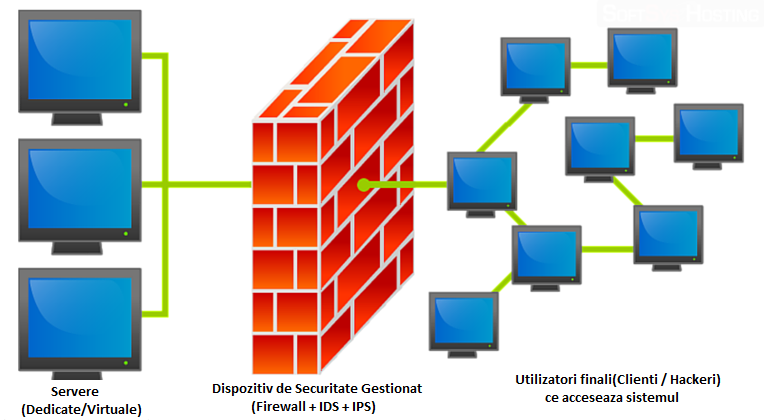
\includegraphics[width=0.6\textwidth]{ips.png}
	\caption{Administrarea securitatii unei aplicatii}
	\label{fig:ips-example}
\end{figure}

Figura ~\ref{fig:ips-example} prezinta administrarea securitatii unei aplicatii folosind combinatia dintre cele trei sisteme. \\

In comparatie cu sistemele de detectie a intruziunilor care sunt sisteme pasive si scaneaza reteaua fara sa interferezu cu traficul, sistemele de prevenire a intruziunilor sunt plasate intre server si cilenti, alterand in mod automat traficul in cazul in care acesta declanseaza una din regulile prezente in sistem. Precum sunt prezentate si in articolul \textbf{What is an intrusion prevention system?} \cite{what_is_ips}, printre functionalitatile unui sistem de prevenire a intruziunilor se numara:
\begin{itemize}
	\item Notificarea unui administrator de retea in cazul in care un sau mai multe reguli sunt declansate.
	\item Oprirea pachetelor considerate malitioase pentru retea.
	\item Blocarea unor utilizatori prin excluderea adreselor ip ale acestora.
	\item Resetarea unor conexiuni.
\end{itemize}

In cea ce priveste functionalitatile oferite de un sistem de prevnire a intruziunilor, acestea sunt specifice tipului sistemului. Conform autorului articoluiui \textbf{Intrusion Prevention System (IPS): Definition \& Types} \cite{ips_types}, Beth Hendricks, exista patru tipuri primare de astfel de sisteme:
\begin{itemize}
	\item Network-based: Protejeaza intraga retea.
	\item Wireless: Protejeaza doar reteaua wireless.
	\item Network behavior: Examineaza traficul din retea.
	\item Host-based: Software cu scopul de a proteja un singur calculator.
\end{itemize}

Sistemele de tipul Network-based(reprezentand si categoria in care se incadreaza  \textit{\thesistitle}) presupun implementarea unor senzori in retea carea captureaza si analizeaza traficul ce trece prin acesta. Acesti senzori sunt plasati in puncte cheie a retelei pentru a putea captura in timp reala traficul, iar in cazul interceptarii unor activitati malitioase sa poata interveni imediat, fara sa scada performanta retelei. Aceste siteme ofera protectie retelei indiferent de dimensiunilie sau cresterea acesteia, adaugarea de noi device-uri fiind posibila fara sa necesite adaugarea de noi senziori. Adaugarea de noi senzori fiind nevoita doar in cazul in care traficul retelei depaseste capacitatea de procesarea a senzorilor curenti, infulentand astfel performantele retelei \cite{impl}.

In functie de nevoi, un sistem de prevenire a intruziunilor poate sa ofere diferite optiuni de protectie pentru diferite parti ale retelei. Unele sunt capabile sa opreasca traficul malitios sau sa limiteze latimea de banda catre anumite parti ale retelei. Conform \cite{ips_sec_types} aceste siteme pot oferi protecti impotriva urmatoarelor tipuri de atacuri:
\begin{itemize}
	\item \textbf{ICMP Storms:} un volum mare de ecouri ICMP pot sa indice activitati malitioase precum cineva ce scaneaza reteaua.
	\item \textbf{Ping to Death:} un utilizator poate sa modifice comanda de ping, astfel incat sa trimita un numar mare de pachete de dimensiune mare catre o destinatie tinta pentru a o scoate din uz.
	\item \textbf{SSL Evasion:} unele atacuri se pot folosi de criptarea SSL pentru a evita dispozitivele de securitate, intrucat in general acestea nu sunt decriptate.
	\item \textbf{IP Fragmentation:} consta in expluatarea faptului ca pachetele sunt descompuse in fragmente pentru a staisface cerintele de dimensiune a retelelor traversate, inundand o destinatie tinta cu fragmente false pentru a ii consuma resursele. 
	\item \textbf{SMTP mass mailing attacks:} un sistem infectat poate sa se foloseasca de de email-ul utilizatorului pentru a se raspandi, rezultand intr-un trafic mare destinat serverului de mail.
	\item \textbf{DoS/DDoS attacks:} cu scopul de a face o resursa indisponibila utilizatorilor, este realizata prin inundarea sistemului tinta cu un numar mare request-uri de la unul sau mai multe(in cazul DoS distribuit - DDoS) siteme malitioase.
	\item \textbf{SYN Flood attacks:} atacatorul trimite un numar mare de pachete de initiare a unei conexiuni fara sa mai raspunda ulterior, epuizand astfel resursele de memorie.
	\item \textbf{Http obfuscation:} pentru a evita sa fie detectate de anumite siteme de protectie, unele atacuri folosesc tehnici de ofuscare a request-urilor HTTP.
	\item \textbf{Port Scanning:} este folosit pentru descoperi ce porturi sunt deschise pe un sistem, ulterior permitandu-i atacatorului sa stie ce vulnerabilitati ar putea prezneta sistemul.
	\item \textbf{ARP Spoofing:} un atacator trimite in retea pachete false de ARP legandu-si propria adresa MAC de adresa IP a unui alt sistem. Ca urmare, atacatorul va primi pachete destinate sistemului cu adresa IP folosita in pachetul de ARP.
	\item \textbf{CGI Attacks:} un atacator poate sa trimita request-uri malitioase, determinand destinatia sa trateze request-ul primit ca si cod executabil, oferindu-i atacatorului acces pe sistem.
	\item \textbf{Buffer Overflow attacks:} presupune ca atacatorul sa depaseasca limitele unui buffer de lungime fixa, excesul de date ajungand sa suprascrie zone adiacente de memorie rezultand in caderea sistemului sau dandu-i atacatorului oportunitatea sa ruleze cod propriu.
	\item \textbf{OS Fingerprinting attacks:} presupune ca atacatorul sa descopere ce sistem de operare ruleaza pe un sistem si folosindu-se de aceasta informatie sa expluateze vulnerabilitati specifice acelui sistem de operare.
\end{itemize}

Sistemul propus, \textit{\thesistitle} implementeaza un sistem de prevenire a intruziunilor folosindu-se de un reverse proxy pentru a intercepta tot traficul care intra si iese din retea( reprezentand senzorii ce au rol de a captura si analiza traficul) si oferind protectie impotriva a doua categorii de atacuri: SQL injection si blocarea traficului venit de la ip-uri ce utilizeara frecvent Tor.

Pentru prevenirea atacurilor de SQL injection, se foloseste o metoda asemanatoare celei propuse de Eun Hong Cheon, Zhongyue Huang si Yon Sik Lee in lucrarea \textbf{Preventing SQL Injection Attack Based on Machine Learning} \cite{sqli_how}. Pentru clasifiacrea request-urilor HTTP in SQL injection sau curate, se foloseste un sistem bazat pe machine learning. Acest sistem este antrnat anterior cu date reale, ca si trasaturi fundamentale in clasificare, folosindu-se cuvintele cheie si simbolurile specifice limbajului SQL(spre exemplu: SELECT, ADD, DELETE, ", ' etc.).

\begin{figure}[h]
\centering
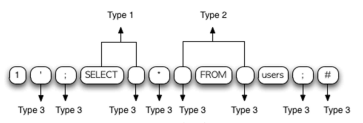
\includegraphics[width=0.6\textwidth]{sqli.png}
\caption{Tipuri de trasaturi ale limbajului SQL}
\label{fig:sql-features}
\end{figure}

Figura ~\ref{fig:sql-features} prezinta tipurile de trasaturi luate in considerare in lucrarea \textbf{Preventing SQL Injection Attack Based on Machine Learning} in raport cu simbolurile sau cuvintele cheie folosite. 


O alta abordare pentru prevenirea atacurilor SQLI este propusa de Fredrik Valeur, Darren Mutz si Giovanni Vigna in lucrarea \textbf{A Learning-Based Approach to the Detection of SQL Attacks} \cite{sqli_how2}. In aceasta lucrarea se prezinta folosirea unui sistem bazat pe detectia de anomalii pentru detectarea atacurilor ce expluateaza o aplicatie pentru a ii compromite baza de date. Asemeni abordarii bazate pe machine learning, acest sistem presupune o faza anterioara de antrenare in care se invata comportamentul normal al utilizatorilor, alcatuind astfel niste profile specifice. Astfel in faza de detectie, comportamentul ce nu coincide cu profilele alcatuite in faza de antrenate, este considerat malitios.

Pentru prevenirea utilizatorilor de Tor, in general lista de ip-uri este alcatuita din toate ip-urile care au utilizat reteaua intr-un anumit interval de timp, aceasta fiind actualizata periodic. O astfel de abordare este folosita si in cazul marelui firewall al Chinei \cite{china_tor} care indentifica nodurile la prima accesare a retelei de Tor. Insa precum precum se evidentiaza si in articolul \textbf{Characterizing the Nature and Dynamics of Tor Exit Blocking} \cite{tor_1} o astfel de abordare nu este cinstita fata de unii utilizatori de Tor, intrucat reputatia acestora este impartita intre toti utilizatorii. Astfel un nod care este utilizat doar pentru cateva minute sau ore(probabil din motive de curiozitate) poate sa ajunga sa fie blocat, fiind tratat asemeni cu un nod ce functionaza de cateva zile. O astfel de discriminare a incercat sa fie evitata prin implementarea aleasa a sistemului propus. Pentru realizarea listei de ip-uri blocate se foloseste un algoritm ce stabileste o limita de timp minima de functionare pentru un anumit nod in intervalul a 30 de zile.


 \section{Tehnici/Tehnologii/Surse folosite}

Pentru realizarea sistemului propus s-au folosit doua limbaje de programare: Pyhton2/3(pentru partea de back end) si C\#(pentru partea de front end). In partea de back end a proiectului se realizeaza implementarea unui reverse proxy pentru a intercepta traficul uneia sau mai multor interfete, un modul pentru clasificarea request-urilor impotriva atacurilor SQL injection si un modul pentru generarea listei negre de ip-uri ce utilizeaza frecvent reteaua Tor. Toate aceste componente sunt realizate prin utilizarea de librarii open-source pentru a usura si eficientiza munca precum: twisted \cite{twisted}, beautiful soup \cite{btf_soup}, libsvm \cite{libsvm}.

Motivul utilizarii atat limbajului Python3 cat si Python2 este datorat diferenteleor de module si librarii open-source disponibile pentru cele doua limbaje dar si a fatului ca suportul pentru Python2 se inchei in anul 2020. Conform documentatiilor oficiale \cite{python3_doc} si \cite{python2_doc}, dar si articolului \textit{Python 2 to python 3: why, and how hard can it be?} de Tim Grey \cite{why_python3}, intre cele doua versiuni nu sunt modificari majore, insa in anumite cazuri pot exista librarii care sa ofere doar suport pentru una dintre aceasta.

In realizarea modulului pentru clasificarea request-urilor impotriva atacurilor SQL injection sa folosit o colectie de date reale atat de atacuri cat si de trafic curat. Pentru uniformizarea acestor date si pentru a trata tentativele de pacalire a clafisicatorului prin codarea unor caractere in valoarea lor in cod hexadecimal (exemplu 'https://www.google.ro /search?q=a' echivalent cu 'https://www.google.ro/search?q=\%61') datele au fost preprocesate si transformate in intregime in coduri hexadecimale \cite{ascii}. In procesarea datelor, petru indetificarea trasaturilor relevant, s-au indentificat caracterele specifice limbajului \cite{char_sql} si cuvintele cheie rezervare \cite{key_sql}. Ulterior, pentru antrenarea modelului de support vector machine si pentru clasificarea noilor request-uri s-a folosit software-ul open-source libsvm \cite{libsvm_class}. 

\begin{figure}[h]
	\centering
	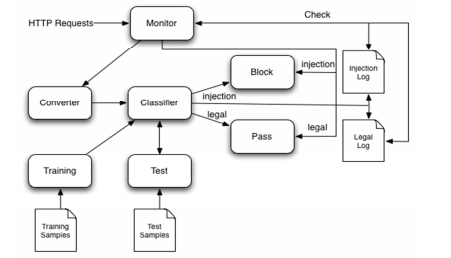
\includegraphics[width=0.6\textwidth]{sql_arh.png}
	\caption{Arhitectura unui sistem de clasificare a request-urilor HTTP}
	\label{fig:sql-arh}
\end{figure}

Figura ~\ref{fig:sql-arh} arhitectura unui sistem de clasificare a request-urilor HTTP de un sistem bazat pe machine learning. Structura este prezentata in lucrarea prezentata si anterior \textbf{Preventing SQL Injection Attack Based on Machine Learning} \cite{sqli_how}. Acesta structura a reprezentat un model de pornire in realizarea modulului de prevenire a atacurilor SQL injection, implementarea modulului incercand sa aduca imbunatatiri de performanta prin modificarea algoritmului folosit pentru antrenarea modelului de support vector machine dar si prin filtrarea trasaturilor propus in lucrare in conformitate cu raportul dintre obijnuinta de aparitie a acestora atat in request-urile ce intentioneaza sa execute un atac cat si in cele curate.

Pentru blocarea ip-urilor utilizate de reteua Tor s-a folosit un script scris in Python3. Programul interogheaza periodic(din 6 in 6 ore) informatiile oferite de \textit{Tor Network Status} \cite{tot_status} indentificand astfel nodurile cu un "Uptime" mai mare de 7 zile in parcursul unei luni. Blocarea ip-urilor se realizeaza prin compoararea cu o astfel de lista generata lunar.

Componenta ce incorporeaza toate modulele de protectie, este cea de reverse proxy. Aici este monitorizat tot traficul ce vine de pe o anumita interfata(una sau mai multe, in functie de configuratia utilizatorului) si este trecut prin toate modulele disponibile pentru a verifica conditiile de securitate. Pentru testarea daca o adresa ip este utilizata frecvent de reteaua Tor, in momentul in care un client doreste sa realizaze o conexiune la server-ul protejat de sistem, adresa ip a acestuia este verificata sa nu se afle pe lista ip-urilor blocate. Pentru actualitate, lista adreselor ip blocate este actualizata periodic cu adresele ip utilizate frecvent de reteaua Tor in ultima luna. Modulul de prevenire a atacurilor SQL injection este integrat tot in componenta de reverse proxy, insa evaluarea request-urilor este facuta dupa realizarea conexiunii intre client si server. Request-urile primite de catre server sunt tratate asemanator celor folosite pentru antrenarea modulului de support vector machine, insa pentru clasificarea acestora este folosit modulul antrenat in faza initiala si software-ul de prezicere oferit tot de libsvm \cite{libsvm}.
	
	

	





